% -*-latex-*-
% Ajouter règle du missing five et des cohortes éteintes tronquées croissantes.
% Document name: /home/brouard/texte/cours/agreg/99/agreg99-1.tex
% Creator: Nicolas Brouard [brouard@brouard.ined.fr]
% Creation Date: Sun Jun  6 08:21:05 1999
% Revised Date: Wed Sep 21 15:50:33 2016

% These lines tell TeXworks to typeset with xelatex, and to open and
% save the source with Unicode encoding.
% !TEX program = pdflatex
% !TEX encoding = UTF-8 Unicode
\documentclass[11pt,a4paper]{article}
\scrollmode
\usepackage{hyperref} %\href{url}{label} or \url{url}
\usepackage{amsmath,color}
\usepackage{unicode-math}
\usepackage[utf8x]{inputenc} %for pdftex engine and unicode characters
\usepackage{graphicx}
\usepackage{natbib} % Put the bibliography as apa
\title{Properties of life left pyramids}
\tolerance 200  % Standard TeX tolerance; could be set to 1000
\author{Nicolas Brouard}
\usepackage[yyyymmdd,hhmmss]{datetime}
\date{\today \,at \currenttime}
\DeclareMathOperator{\e}{e}
\DeclareMathOperator{\E}{E}
\DeclareMathOperator{\Res}{Res}
\def\D{{\,\mathrm d}}
\bibliographystyle{abbrvnat}
  \begin{document}
 \maketitle
\bibliographystyle{abbrvnat}
Let us consider a state $s$ for a multistate population, and $a$ being the age in last state $s$ or time spent the last entry in state $s$. 
\begin{enumerate}
\item  The population density $p(t,a)$ at time $t$ and age $a$ can be
  defined as the population that, at time $t$, has an age between $a$
  and $a + \D a$\,. Prove that this number is also equal to the
  population that has reached age $a$ between time $t$ and
  $t-\D a$\,\citep{Brouard-Iford-Mouvements}.  
\item We are now considering a closed population which is defined by
  the absence of migration.  $P(t)=\int_0^∞ p(t,u) \D u)$, is the size
  of the total population at a census occurring at exact time $t$ and
  let us consider its sub-population $P(t,a)=\int_0^a p(t,u)\D u$
  under age $a$\,.  Let us suppose that the next census is at time
  $t+a$ (see Fig.~\ref{f:life-left-stable-multi-lexis-ipe}),
 \begin{figure}[htbp]\centering
   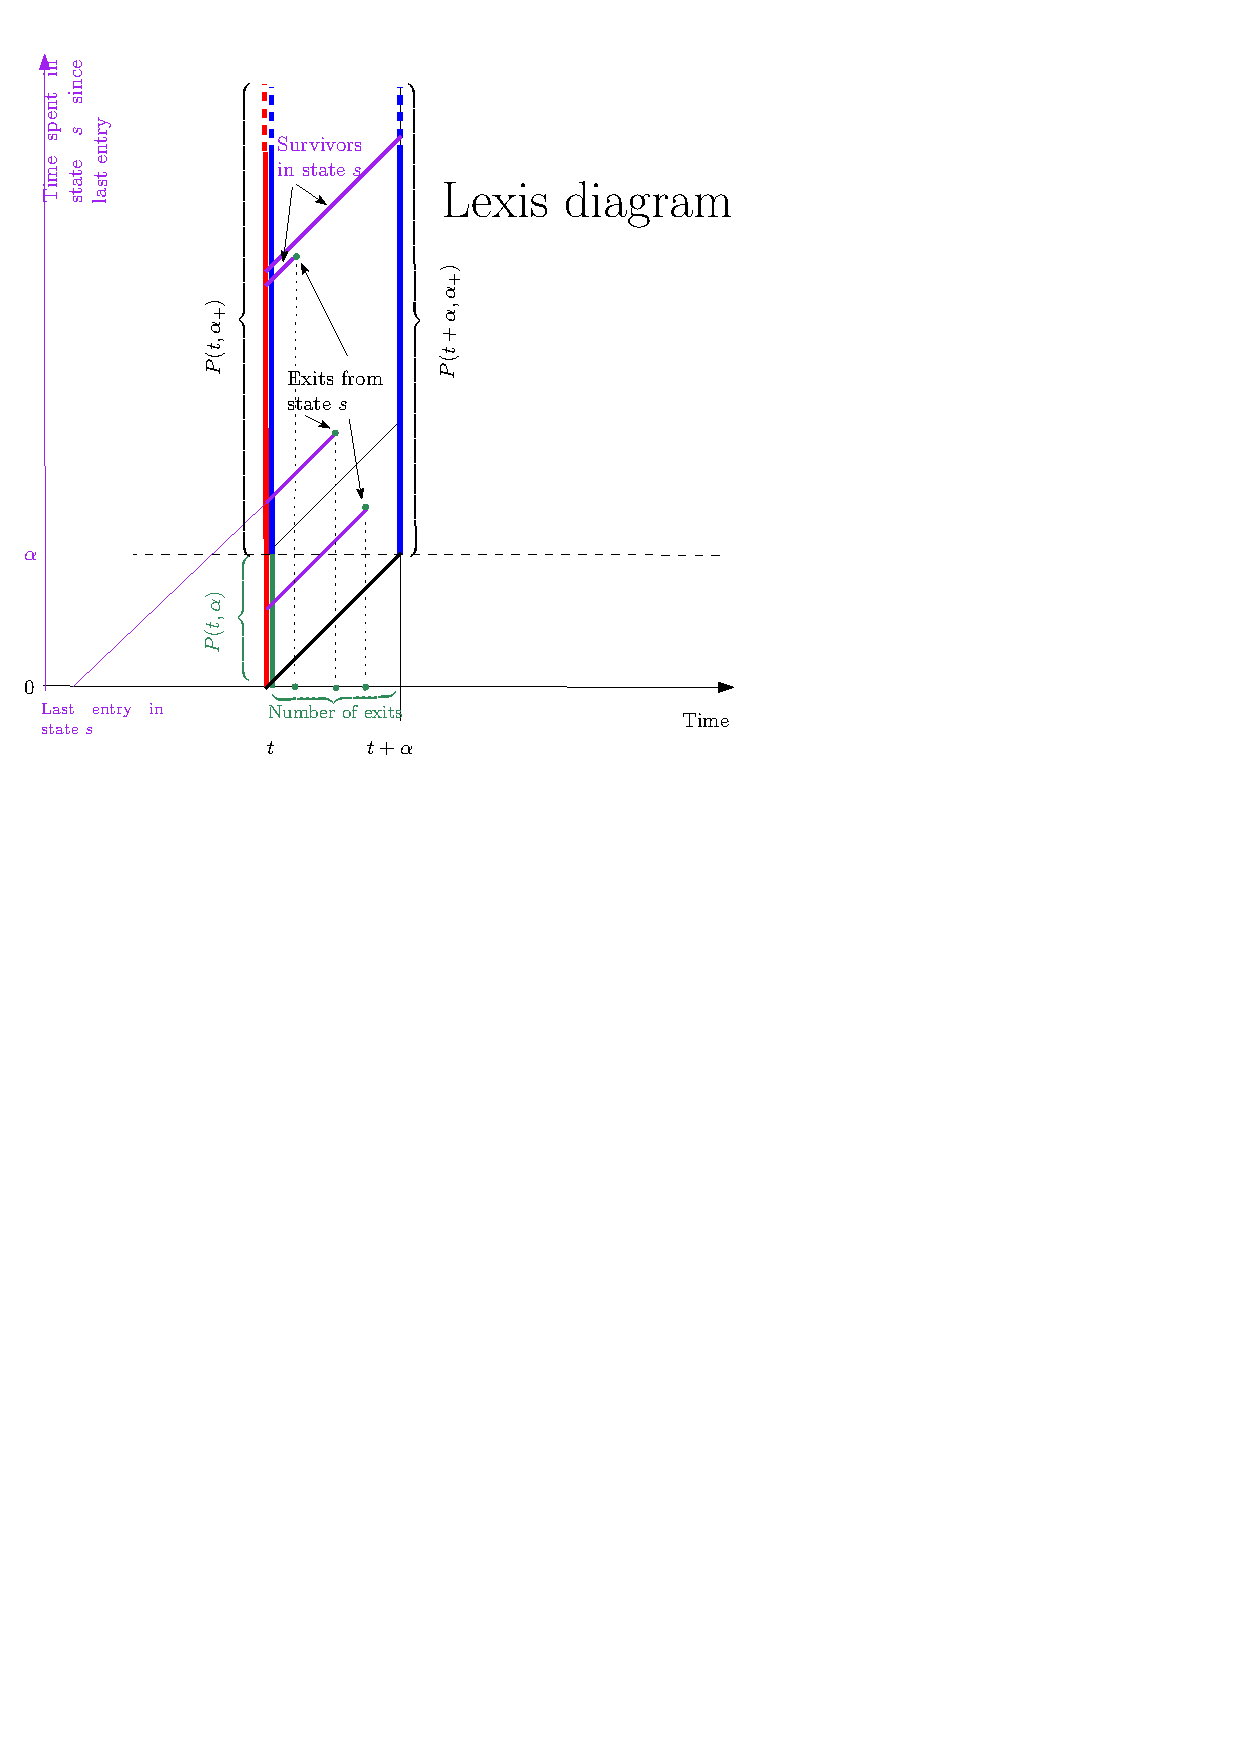
\includegraphics[width=.8\textwidth]{life-left-stable-multi-lexis-ipe}
   \caption{\sf Lexis diagram showing the population at two censuses
     spaced at $\alpha$ years and sub-populations of less than $\alpha$
     years and more than $\alpha$ years\,.}\label{f:life-left-stable-multi-lexis-ipe}
 \end{figure}
 and consider the sub-population $P(t+a, a_+)$ of more than $a$ years
 at the new census, $P(t+a, a_+)=\int_a^∞ p(t+a,u) \D u)$. Deduce that
 the difference between both populations $P(t,a)-P(t+a, a_+)$
 corresponds to the number of exits from state $s$ occurring in
 population $P(t)$ between the two censuses.

\item We are now considering a stationary multistate population: a
  population with constant force of interaction between states over
  time and constant number of entries in each states by time unit. Let
  us denote $n$ for the state $s$ considered. Its population
  ``density'' at time $t$ and age $a$ is then $p(t,a)\D a =nl(a) \D a$
  and is independent of time $t$ where $l(a)$ is the survivorship in
  state $s$\,. We are neglecting stochastic variations by considering
  huge populations.
\item Deduce from previous result that in a multistate stationary population,
  there are exactly the same number of people having lived $a$ years in a state
  than people having $a$ years to live in this state. And therefore prove that both,
  pyramids by time spent in a state and by time to live in this state, are identical.
\item Stable multistationary state: suppose now than $n$ is increasing or decreasing exponentially: $n(t)=n_0\exp(\rho t)$, etc.
\end{enumerate}

\end{document}
%
% These lines tells gnu-emacs to typeset with the xetex engine
% which requires Unicode encoding only (utf-8)
% ^c^t^s for toggling synctex. 
% ^-Shift-Click to move from pdf to source, Command-Shift-Click on OSX
%%% Local Variables:
%%% TeX-engine: xetex
%%% TeX-source-correlate-method-active: synctex
%%% ispell-local-dictionary: "american"
%%% coding: utf-8
%%% End:




